%%
% BIThesis 本科毕业设计论文模板 —— 使用 XeLaTeX 编译 The BIThesis Template for Undergraduate Thesis
% This file has no copyright assigned and is placed in the Public Domain.
%%

% 第一章节
\chapter{实验设计与结果分析}

\section{实验设计}

\subsection{开发环境配置}

\textcolor{black}{实验使用如下开发环境:}

\textcolor{black}{(1)实体机操作系统及版本号:Windows10 22H2}

\textcolor{black}{(2)虚拟机软件,虚拟机操作系统:VMWare Workstation 16.1.2 build-17966106,Windows7 旗舰版
}

\textcolor{black}{(3)集成开发环境:PyCharm 2024.3.5 (Professional Edition) }

\textcolor{black}{(4)Python虚拟环境:Anaconda 24.11.3 AnacondaNavigator2.6.5 }

\textcolor{black}{(5)反病毒软件:主机安装Clam AV,建议手动更新病毒库到最新版本。虚拟机中安装火绒杀毒和360杀毒以备后续使用,本实验中不建议在主机上安装多个反病毒软件,因为可能会导致主机出现蓝屏崩溃问题,因此,其它用于后续使用的反病毒软件建议安装在虚拟机中。}

\textcolor{black}{(6)项目依赖位于项目根目录下的requirements.txt文件中,可以使用anaconda直接导入requirements.txt文件来创建Python虚拟环境。}

\textcolor{black}{(7)实体机存储:内存空间 32GB,磁盘空间 512GB}

\subsection{原始样本获取}

\textcolor{black}{首先,在开始实验前,需要提前收集足够量的恶意样本以供本实验使用,针对此问题的解决方案是从国外VirusShare的开放恶意样本库,以及部分国内安全软件论坛,例如火绒杀毒,360杀毒等官方论坛,收集并且下载恶意样本。本实验中大约使用2000个恶意样本,并将它们分为五组以备后续使用。如果是在Virus Share上收集,需要注意文件的类型,需要是PE可执行文件。}

\textcolor{black}{用于对抗性操作的无害程序,主要用于增加伪造的签名,无害段等对抗性操作,这些无害程序的获取方式,可以从国内一些软件公司的软件安装包获取,使用sigthief将签名剥落,关于sigthief的具体使用可以参考https://github.com/secretsquirrel/SigThief 的readme的相关说明,这些从良性程序剥落下的签名可以从一些官方途径下载的软件安装包可执行文件中剥落下来。用于增加无害段需要收集一些良性DLL文件,可以从Windows操作系统根目录下的一些DLL文件中获取。}

\subsection{配置VMWare虚拟机}

\textcolor{black}{需要创建实验用Windows7虚拟机并安装VMware Tools,并调整360杀毒相关设置关闭不需要的反病毒引擎,取消勾选系统修复引擎、behavioral脚本引擎,鲲鹏引擎,避免对实验结果造成干扰。同时,需要注意潜在的样本污染问题,对于360杀毒,需要关闭自动上传发现的可疑文件,取消勾选自动上传发现的可疑文件,否则可能导致有些样本被360杀毒上传到云查杀服务器数据库中,导致后续结果查杀率偏高的问题。}

\textcolor{black}{需要注意的是,安装360杀毒后需要重启虚拟机以保证360杀毒相应查杀服务开启,否则会导致实验结果出现偏差。}

\textcolor{black}{本实验不会测试360杀毒的鲲鹏引擎,是因为大多数反病毒软件,倾向于防御现有的威胁和威胁变种,而不是没有广泛传播的对抗性样本,鲲鹏引擎也如此,它多被360杀毒用于对抗目前广泛流行的恶意样本(例如银狐和某些流行的勒索病毒),而非对抗性样本或是离目前时间较久远的样本,而且鲲鹏引擎几乎没有机器学习的自学习能力,但QVM引擎具有机器学习能力,很明显,QVM引擎更适合用于本次实验的结果检验。这是因为有时需要反病毒软件对未知程序的判断更加精准以及判断速度更快,也就是尽量降低误报的可能性以及判断时间。为了减少误报率,很多反病毒软件厂商可能会使用白名单数字签名放行,或是使用文件哈希白名单来进行放行。因为例如Intel、AMD的硬件驱动程序,它们会加载驱动,如果这些硬件外设驱动程序因为释放了一些驱动文件被反病毒软件误报没有放行,将会导致某些外设驱动不能正常安装,对用户来说后果无疑是灾难性的,极有可能导致操作系统或是计算机崩溃。但这些硬件驱动程序跟某些病毒的行为很相似,某些病毒也会使用驱动来提升自己的操作权限,使自己具有更强的破坏力以及更好地针对和破坏反病毒软件,因此,对于这些驱动程序以及一些驱动安装工具,大多数反病毒软件会选择单独白名单规避此类问题。同时,360杀毒的behavioral脚本查杀引擎和系统修复引擎也需要关闭防止造成检出率偏高导致误差。}

\subsection{结果评估标准}

\textcolor{black}{首先,定义查杀率如下:}

\textcolor{black}{查杀率计算公式如式4-1:}
\begin{equation}
P_{detect\_rate}=m_{detect\_sample\_amount}/m_{total\_sample\_amount}
\end{equation}

\textcolor{black}{对于某个恶意软件集合$sample\ s_{\omega}$,某反病毒软件的查杀率被定义为经该反病毒软件扫描该恶意软件样本集合的检出恶意软件数量除以恶意软件集合中总恶意软件数量。}

\textcolor{black}{为了更好计算样本集的规避反病毒软件的查杀效果,使用该公式要求原始样本和生成的对抗性样本前后都使用同一款反病毒软件进行扫描,则查杀下降率定义如式(4-2)所示:}
\begin{equation}
\delta_{decline\_rate}=(P_{detect\_rate\_before}-P_{detect\_rate\_after})/P_{detect\_rate\_before}
\end{equation}

\textcolor{black}{语言描述为:查杀下降率=(原始样本检出率-处理后样本检出率)/原始样本检出率。}

\textcolor{black}{Virus Total检出率的定义为式(4-3)所示: }
\begin{equation}
P_{detect\_rate}=m_{detect\_engine\_amount}/m_{total\_engine\_amount}
\end{equation}

\textcolor{black}{对于某个恶意软件样本,VirusTotal检出率定义为检出引擎总数/Virus Total扫描引擎总数。}

\textcolor{black}{Virus Total检出率的下降率定义如式(4-4)所示:}
\begin{equation}
    \delta_{decline\_rate}=(P_{detect\_rate\_before}-P_{detect\_rate\_after})/P_{detect\_rate\_before}
\end{equation}

\textcolor{black}{对于某个恶意软件样本,VirusTotal检出率的下降率定义为(原始样本VirusTotal检出率-处理后样本VirusTotal检出率)/原始样本VirusTotal检出率。}

\section{实验结果}

\textcolor{black}{在本次实验中,一共使用了五组样本集,合计大约2000个样本来进行测试,测试结果如下所示。对于处理前的原始样本集和处理后的样本集,分别使用前文中配置好的恶意程序扫描模块和手动上传至虚拟机使用火绒杀毒和360杀毒扫描,并且随机选取一些原始样本和对应的处理后样本上传VirusTotal进行分析。值得注意的是,获取实验结果数据时,在虚拟机中使用360杀毒和火绒对样本扫描之前,需要关闭虚拟机中的反病毒软件,再在主机上使用XFTP等软件或VMwareTools拖拽向虚拟机中发送样本集,防止样本集发送过程中受到反病毒软件的干扰和潜在的数据污染问题,例如360杀毒会默认禁止存在风险的远程主机向本主机的FTP协议,在本次实验中对于虚拟机我们不需要这个防御功能。且在主机和虚拟机的FTP协议或VMWareTools拖拽完成文件传输后,虚拟机接收到文件后,360杀毒会自动扫描文件,这是不应该被允许的。因为会导致后续检出率偏高以及360杀毒等反病毒软件会直接隔离虚拟机接收到的样本集中的一些样本,对后续统计查杀数量带来了不便。}

\subsection{实验结果的数据图示}

\textcolor{black}{五组样本集处理前后的扫描结果图\ref{fig:sample1}、图\ref{fig:sample2}、图\ref{fig:sample3}、图\ref{fig:sample4}、图\ref{fig:sample5}、图\ref{fig:Virus_Total}、图\ref{fig:compare_with_different_model}所示,对其具体分析将在后续章节中进行。}

\begin{figure}
  \centering
  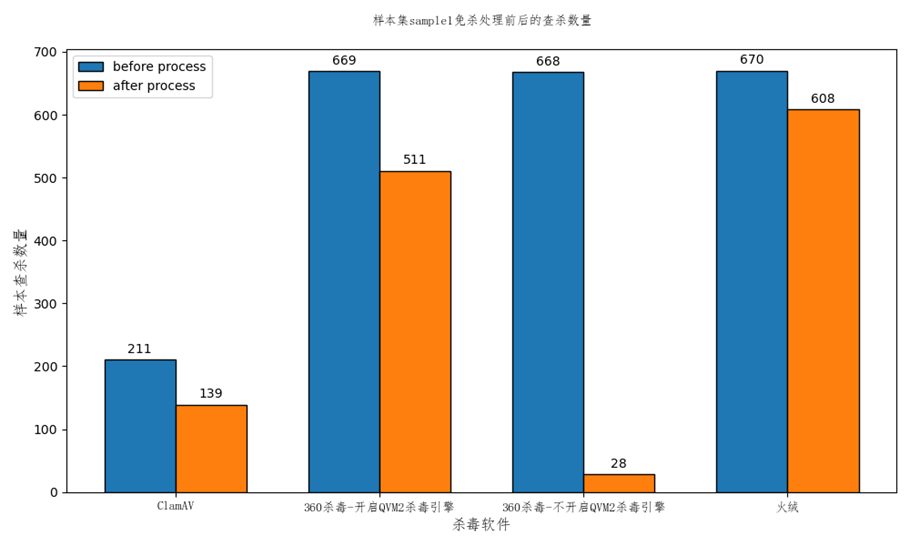
\includegraphics[]{images/sample1.png}
  \caption{sample1}\label{fig:sample1}
\end{figure}

\begin{figure}
  \centering
  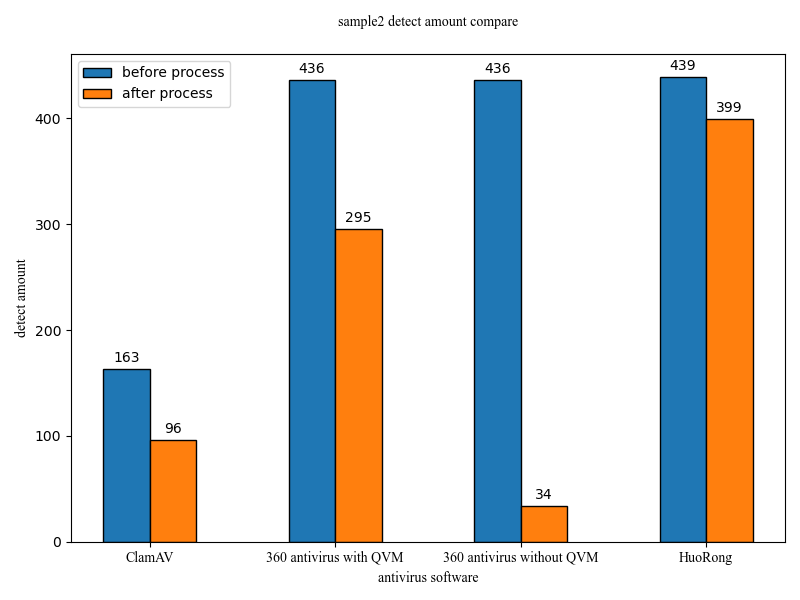
\includegraphics[]{images/sample2.png}
  \caption{sample2}\label{fig:sample2}
\end{figure}

\begin{figure}
  \centering
  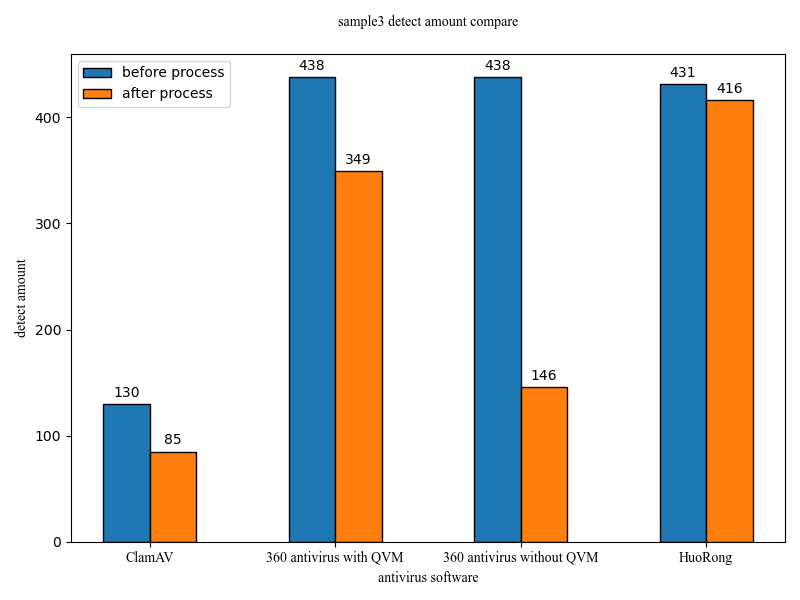
\includegraphics[]{images/sample3.png}
  \caption{sample3}\label{fig:sample3}
\end{figure}

\begin{figure}
  \centering
  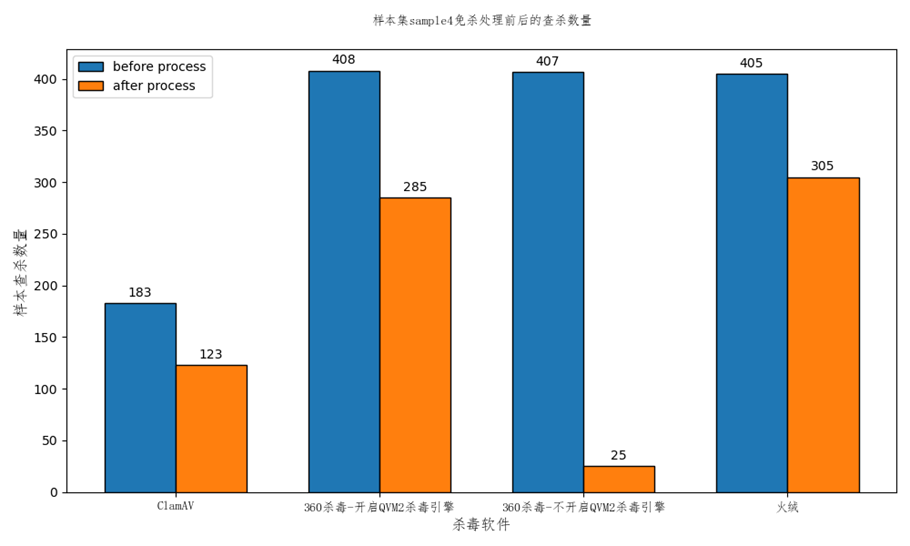
\includegraphics[]{images/sample4.png}
  \caption{sample4}\label{fig:sample4}
\end{figure}

\begin{figure}
  \centering
  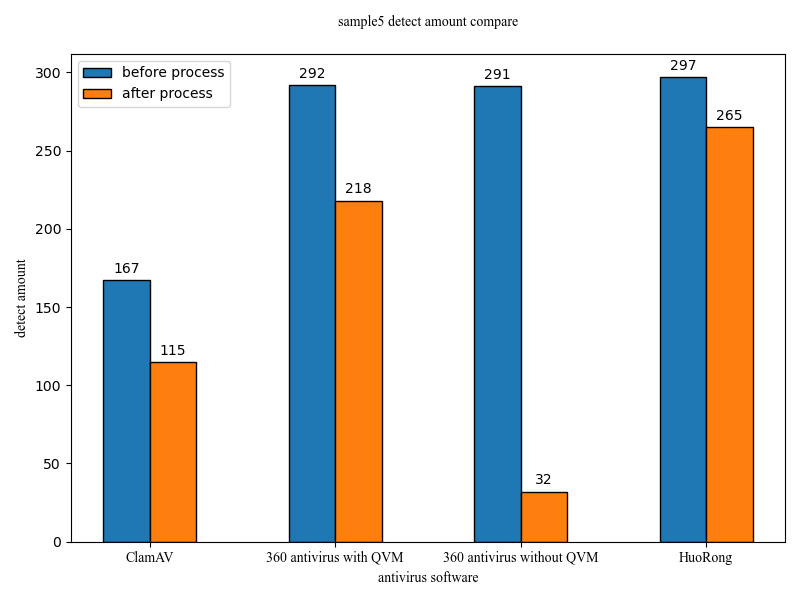
\includegraphics[]{images/sample5.png}
  \caption{sample5}\label{fig:sample5}
\end{figure}

\begin{figure}
  \centering
  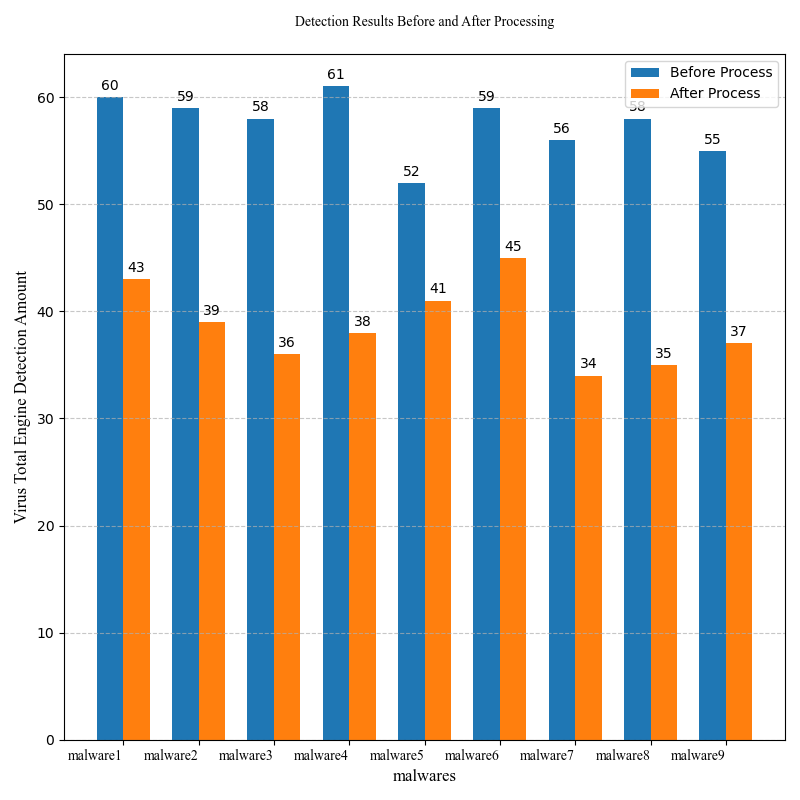
\includegraphics[]{images/Virus_Total.png}
  \caption{Virus Total}\label{fig:Virus_Total}
\end{figure}

\begin{figure}
  \centering
  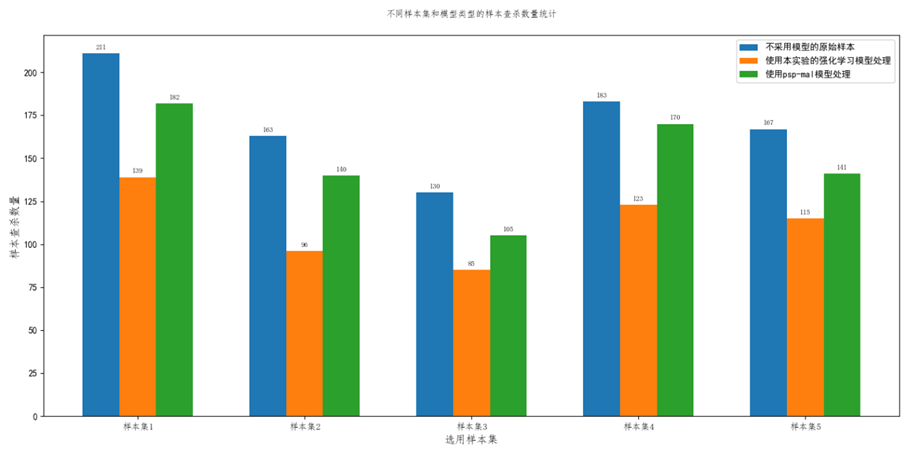
\includegraphics[]{images/compare_with_different_model.png}
  \caption{不同模型ClamAV检出对比}\label{fig:compare_with_different_model}
\end{figure}

\subsection{检出率及其变化的计算}

\textcolor{black}{首先,对于某组样本中的随机抽样的部分程序,笔者使用了Virus Total来进行上传扫描。}

\textcolor{black}{经过对图\ref{fig:sample1},图\ref{fig:sample2},图\ref{fig:sample3},图\ref{fig:sample4},图\ref{fig:sample5}中的数据进行计算,可以发现:}

\textcolor{black}{(1)对于样本集sample1:}

\textcolor{black}{Clam AV对本实验强化学习模型处理前后的样本检出率从31.3\%下降到了20.7\%;开启QVM杀毒引擎的360杀毒对本实验强化学习模型处理前后的样本检出率从99.3\%下降到了75.8\%;只开启360云查杀引擎,不开启QVM杀毒引擎的360杀毒对强化学习模型处理前后的样本检出率从99.1\%下降到了4.2\%;火绒杀毒对本实验强化学习模型处理前后的样本检出率从99.4\%下降到了90.2\%。}

\textcolor{black}{(2)对于样本集sample2:}

\textcolor{black}{Clam AV对本实验强化学习模型处理前后的样本检出率从37.4\%下降到了22.0\%;开启QVM杀毒引擎的360杀毒对本实验强化学习模型处理前后的样本检出率从100\%下降到了67.7\%;只开启360云查杀引擎,不开启QVM杀毒引擎的360杀毒对本实验强化学习模型处理前后的样本检出率从100\%下降到了7.8\%;火绒杀毒对本实验强化学习模型处理前后的样本检出率从100\%下降到了91.5\%。}

\textcolor{black}{(3)对于样本集sample3:}

\textcolor{black}{Clam AV对本实验强化学习模型处理前后的样本检出率从29.5\%下降到了19.3\%;开启QVM杀毒引擎的360杀毒对本实验强化学习模型处理前后的样本检出率从99.5\%下降到了79.3\%;只开启360云查杀引擎,不开启QVM杀毒引擎的360杀毒对本实验强化学习模型处理前后的样本检出率从99.5\%下降到了33.2\%;火绒杀毒对本实验强化学习模型处理前后的样本检出率从98.0\%下降到了94.5\%。}

\textcolor{black}{(4)对于样本集sample4:}

\textcolor{black}{Clam AV对本实验强化学习模型处理前后的样本检出率从44.9\%下降到了30.1\%;开启QVM杀毒引擎的360杀毒对本实验强化学习模型处理前后的样本检出率从100\%下降到了69.9\%;只开启360云查杀引擎,不开启QVM杀毒引擎的360杀毒对本实验强化学习模型处理前后的样本检出率从99.8\%下降到了6.1\%;火绒杀毒对本实验强化学习模型处理前后的样本检出率从99.3\%下降到了74.8\%。}

\textcolor{black}{(5)对于样本集sample5:}

\textcolor{black}{Clam AV对本实验强化学习模型处理前后的样本检出率从57.2\%下降到了39.7\%;开启QVM杀毒引擎的360杀毒对本实验强化学习模型处理前后的样本检出率从100\%下降到了74.7\%;只开启360云查杀引擎,不开启QVM杀毒引擎的360杀毒对本实验强化学习模型处理前后的样本检出率从99.7\%下降到了11.0\%;火绒杀毒对本实验强化学习模型处理前后的样本检出率从100.0\%下降到了90.8\%。}

\textcolor{black}{根据查杀下降率的定义,对于五个样本集合的查杀下降率计算结果如下表\ref{chart1}中所示: }

\begin{table}[htbp]
  \centering
  \caption{查杀下降率结果}\label{chart1}
  \begin{tabular}{*{6}{>{\centering\arraybackslash}p{2cm}}} \toprule
    反病毒软件类型/样本    & sample1    & sample2    & sample3   & sample4    & sample5   \\ \midrule
    ClamAV    & 34.1\%  & 41.1\% & 34.6\%  & 32.8\%  & 31.1\%\\ \midrule
    360杀毒开启云查杀引擎和QVM引擎   & 23.6\%  & 32.3\%  & 20.3\%  & 30.1\%    & 25.3\%\\ \midrule
    360杀毒开启云查杀引擎不开启QVM引擎 & 95.8\%  & 92.2\%  & 66.7\%  & 93.9\%    & 89.0\%\\  \midrule
    火绒 & 9.3\%  & 9.1\%  & 3.5\%  & 24.7\%    & 10.8\%\\ \bottomrule
    \end{tabular}
\end{table}

\textcolor{black}{计算平均值如表\ref{chart2}中所示:}

\begin{table}[htbp]
  \centering
  \caption{查杀下降率结果平均值}\label{chart2}
  \begin{tabular}{*{2}{>{\centering\arraybackslash}p{2cm}}} \toprule
    ClamAV    & 34.74\%\\ \midrule
    360杀毒开启云查杀引擎和QVM引擎   & 26.32\%\\ \midrule
    360杀毒开启云查杀引擎不开启QVM引擎 & 87.52\%\\  \midrule
    火绒 & 11.48\%\\ \bottomrule
    \end{tabular}
\end{table}

\textcolor{black}{从结果中看出,对抗性样本对于不同反病毒软件的有效性,对360云查杀引擎最有效,对火绒的有效性最差。}

\textcolor{black}{前文中图\ref{fig:Virus_Total}使用Virus Total扫描上传从某个样本集合内随机抽样的PE恶意程序,在云端总共使用了70余个反病毒软件进行分析。}

\textcolor{black}{处理前后检出率变化以及检出下降率变化如表\ref{chart3}所示:}

\begin{table}[htbp]
  \centering
  \caption{查杀下降率结果平均值}\label{chart3}
  \begin{tabular}{*{4}{>{\centering\arraybackslash}p{2cm}}} \toprule
    样本/检出率    & 处理前检出率  & 处理后检出率  & 检出下降率\\ \midrule
    malware1   & 83.3\%  & 59.7\%  & 28.3\%\\ \midrule
    malware2 & 80.8\%  & 54.2\%  & 33.0\%\\  \midrule
    malware3 & 79.5\%  & 50\%  & 37.1\%\\  \midrule
    malware4 & 83.6\%  & 53.5\%  & 36.0\%\\  \midrule
    malware5 & 71.2\%  & 56.9\%  & 20.0\%\\  \midrule
    malware6 & 81.9\%  & 61.6\%  & 24.8\%\\  \midrule
    malware7 & 77.8\%  & 47.2\%  & 39.3\%\\  \midrule
    malware8 & 80.6\%  & 48.6\%  & 39.7\%\\  \midrule    
    malware9 & 75.3\%  & 51.4\%  & 31.8\%\\ \bottomrule
    \end{tabular}
\end{table}

\textcolor{black}{且经过统计,当最大允许处理次数设置为16时,对于样本集sample1的处理总共花费12463.1秒,对于单个样本的平均处理时间为18.49秒。}

\textcolor{black}{样本集1样本大小变化率的散点图如图\ref{fig:scatter_of_sample1}所示,大小变化率的定义为对于某个确定的样本,其处理后的大小除以处理前的大小,可以发现,有少数处理后的样本大小变的较大,甚至可能会达到1000倍以上,这可能是因为添加节所选取的良性DLL文件中的.text节过于庞大导致的。}

\begin{figure}
  \centering
  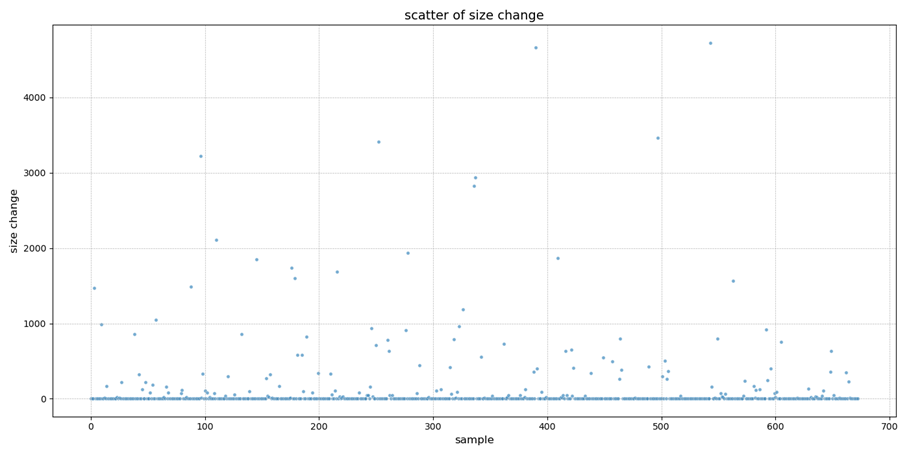
\includegraphics[]{images/scatter_of_sample1.png}
  \caption{scatter of sample1}\label{fig:scatter_of_sample1}
\end{figure}

\subsection{不同反病毒软件对于检出率变化的影响}

\textcolor{black}{处理后的样本对于火绒杀毒来说,表\ref{chart1}中数据计算出的逃逸概率低的原因是火绒有一定的反扰动能力,处理后的样本很多都会判断为:病毒类型-代码混淆器,火绒认为处理后的样本的某些特征是为了规避静态检测过程。说明有一部分反病毒软件的静态特征分析能力,能识别出对抗样本中的扰动。这也是为什么采用Sarsa算法不宜设置过大的state数值的原因,一方面是处理前后的PE程序反复读写,当程序大小因为新增节,新增无意义尾部内容,用无意义字节填充空洞等操作多次使用后变的过于庞大(在某次样本处理时,笔者观察到了一个PE程序处理前后,变为原大小大约6.6倍,从2.67 MB变成了17.6MB),如果不限制state值,程序中途会变得很大,不但导致后续的对抗性样本生成的干扰操作极其缓慢,因为要先读取原文件,然后再加以修改,最后写入磁盘中,Python对于文件的操作是很缓慢的。而且会导致根据查杀结果获取result的速度相当慢,因为Clam AV反病毒软件扫描一个样本的时间也和样本大小正相关,当样本很大的时候,判断查杀结果会相当的慢。另一方面,就是当无意义尾部内容过多,会被反病毒软件认为是疑似恶意程序刻意扰动,从而直接判定此程序为为了绕过反病毒软件检查的恶意程序。而从火绒杀毒对于样本的描述也可以看到这一点,火绒杀毒认为经过处理后的某些恶意程序是代码混淆器。同时,火绒查杀结果总数量会略高于样本数量,原因目前未知。}

\textcolor{black}{同样对于Clam AV,可知它的部分检测也能识别对抗样本中的扰动性操作,尽管经过处理后的恶意程序中有大量良性内容,但Clam AV仍然会查杀这些恶意程序。}

\textcolor{black}{由此可见,部分反病毒软件对于静态规避操作的对抗性扰动有一定的抵抗,会造成处理前后检出率变化较小。}

\textcolor{black}{但QVM引擎对于对抗性扰动能力偏弱,这是因为QVM引擎作为一个自学习的人工智能引擎,这个病毒检测引擎是基于机器学习的模型,通过检测文件的某些特征,来判断该文件是否是恶意程序,如果某程序被QVM引擎检测出是恶意程序,那么360杀毒在查杀结果中会报HEUR/QVM.xx.Malware.Gen字样。这里使用QVM引擎作为检测标准是为了研究论文中的强化学习对抗性样本生成模型产生的处理后静态检测规避对抗性样本在基于不同模型的反病毒软件之间的逃逸可迁移性,以及验证机器学习的病毒检测引擎对于静态检测规避对抗性样本的抗干扰能力。但遗憾的是,QVM引擎对于静态检测规避对抗性样本的抗干扰能力比较差,有时甚至仅仅增加了无意义的图标ICO资源,QVM引擎就认为样本是良性的。}